\documentclass{article}
% Anonymous NeurIPS 2026 submission format. For a double-blind workshop,
% replace the next line by \usepackage[dblblindworkshop,nonatbib]{neurips_2026}
% and set \workshoptitle{<workshop name>} below.
\usepackage[nonatbib]{neurips_2026}
% \workshoptitle{Workshop name}
\usepackage[utf8]{inputenc}
\usepackage[T1]{fontenc}
\usepackage{microtype}
\usepackage{graphicx}
\usepackage{booktabs}
\usepackage{amsmath,amssymb,amsfonts}
\usepackage[hidelinks]{hyperref}

\title{Semantic Flow Under Obfuscation:\\What Code Models Represent, What Survives, and What Becomes Sayable}
\author{Anonymous Author(s)}

\begin{document}
\maketitle

\begin{abstract}
Security analyses need relations that are not properties of individual tokens, such as whether untrusted input reaches a sensitive call. We study whether pretrained code models make this source-to-sink relation accessible, whether access survives semantics-preserving rewrites, and whether the relation aligns with the models' own security vocabulary. We build 480 matched Python programs crossing three sink families and four flow structures. On clean programs, frozen linear readouts reach 0.997--1.000 training accuracy and 1.000 held-out accuracy in DeepSeek-Coder 1.3B, DeepSeek-Coder 6.7B, and StarCoder2-3B, while local-token, whole-program lexical, and embedding controls remain near chance. Atomic obfuscations reveal a selective failure: opaque predicates and mixed Boolean--arithmetic encoding cost exactly zero, renaming has a modest cost, but control-flow flattening alone reduces accuracy to 0.660--0.688. The full four-step composition is no worse beyond measured draw variation. Moreover, 46--56\% of flattened safe/unsafe pairs receive the same prediction, showing that aggregate accuracy overstates retained relational information. Finally, explicit words such as \emph{unsafe} do not consistently carry the distinction, although a label-defined distributed vocabulary direction generalizes to all held-out pairs. These results suggest that code models construct a useful semantic-flow representation, but one tied to source-level control-flow presentation and distributed rather than cleanly verbalized.
\end{abstract}

\section{Introduction}
Program analysis depends on relations. A token may denote a variable bound in an outer scope, a use may depend on a distant definition, and a sensitive argument may be derived from untrusted input. None of these facts can be read reliably from the token alone. If code models represent such relations, their hidden states may support grounded reasoning for security tasks. If they instead rely on names, nearby syntax, or generator regularities, strong clean-code scores may give a misleading picture.

Even a real clean-code representation need not be invariant to different presentations of the same computation. This matters in security: transformations used for packing, evasion, or software protection preserve execution while changing the structure visible in source or intermediate code. Prior probing work asks what code-model states contain \cite{troshin2022probing,chen2022cat}; recent work also shows that obfuscation can reduce end-to-end vulnerability or malware detection \cite{li2025obfuscation,boke2025camouflage}. We connect these questions by auditing the internal relation needed for a simple security analysis.

Our target is precise: at the argument of a code-bearing sink, is the value derived from an untrusted source? We use matched programs in which the unsafe and safe members contain the same source, trusted alternative, propagation, and sink; only the final selected value differs. A frozen linear readout is trained on clean states and tested without refitting. Local token IDs, whole-program n-grams, and the embedding layer provide measured floors. We then apply identifier renaming, opaque predicates, mixed Boolean--arithmetic (MBA) expression encoding, and control-flow flattening both alone and cumulatively. Atomic evaluation is important: a cumulative ladder can locate when a failure appears, but cannot identify which rewrite causes it.

We make three contributions. First, source-to-sensitive-sink flow becomes almost perfectly linearly accessible after contextual computation in three code models, beyond the measured textual controls. Second, atomic attribution shows that flattening alone accounts for the robustness collapse; two visually substantial obfuscations have no measurable cost in isolation. Third, the distinction has a reproducible distributed projection into output coordinates but is not aligned with an obvious security word. The combined result is neither ``models only memorize API names'' nor ``models perform normalized static analysis.'' Instead, these models form relational states over familiar source structure, and those states can fail when the same computation is presented through a dispatch loop.

\section{Benchmark and Method}
\subsection{What we mean by semantic}
We use \emph{semantic} in a controlled and limited sense: a target depends on a program relation, while named surface alternatives are held fixed or measured. For example, the two snippets below contain the same final token \texttt{x}, but it resolves to different definitions.
\begin{center}
{\ttfamily\scriptsize
\begin{tabular}{ll}
\# outer binding & \# inner binding\\
x = 3 & x = 3\\
def f(): & def f():\\
\quad y = 7 & \quad x = 7\\
\quad return x & \quad return x
\end{tabular}}
\end{center}
Earlier experiments in this codebase use such minimal pairs for binding and def--use. Their exact local floor is 0.5, while contextual readouts approach 0.99. We use this as a foundation: the present paper asks whether a security-relevant relation built from the same primitives is accessible and robust. High probe accuracy establishes accessible information, not that a model executes a sound analyzer or causally uses the decoded direction \cite{hewitt2019control}.

\subsection{Matched source-to-sink programs}
The benchmark contains
\[
3\text{ sink families}\times4\text{ structures}\times20\text{ bases}\times2\text{ labels}=480
\]
Python programs. The sink families are command execution, SQL execution, and dynamic-code execution. The structures are a direct flow, a two-assignment chain, a branch merge, and one helper-function boundary. Each base yields an unsafe and safe member. Both include an untrusted source and a trusted literal; the only semantic contrast is which value reaches the marked sink argument. Here ``safe'' means only that this argument receives the independent trusted value. It is not a claim that a general sanitizer makes arbitrary dynamic execution safe.

We split by base, never by program: 168 bases (336 programs) are used for training and 72 bases (144 programs) are held out. This prevents the two members of a pair from crossing the split. Ground truth must agree between restricted instrumented execution and an independent AST taint fixpoint. Sensitive APIs are replaced by recorder stubs, so no command, query, or dynamic code is executed.

\paragraph{Notation.}
Let $b\in\mathcal{B}$ index a semantic base and let
$p_b^1$ and $p_b^0$ denote its unsafe and safe programs. Their labels are
$y(p_b^1)=1$ and $y(p_b^0)=0$. Apart from the final value selected for the
sink argument, the two programs share the same source, trusted alternative,
propagation structure, and sensitive API. For model $m$, layer $\ell$, and
measurement site $s$, we write
\begin{equation}
  h_{m,\ell,s}(p)\in\mathbb{R}^{d_m}
  \label{eq:hidden}
\end{equation}
for the contextual hidden state. This pair notation is used throughout: all
splits, resampling, and robustness comparisons keep $p_b^1$ and $p_b^0$
together.

\subsection{Readouts and controls}
For each model and layer, we extract the hidden state at the sensitive argument and fit a regularized linear classifier using grouped cross-validation on clean training bases. We select one clean layer per model and freeze both layer and classifier before evaluating held-out transformations. We study DeepSeek-Coder 1.3B and 6.7B \cite{guo2024deepseek} and StarCoder2-3B \cite{lozhkov2024starcoder2}.

More precisely, for each candidate layer we fit logistic regression
\begin{equation}
 \hat{y}_{m,\ell}(p)=
 \mathbb{I}\!\left[\sigma\!\left(w_{m,\ell}^{\top}
 h_{m,\ell,s}(p)+c_{m,\ell}\right)\geq\tfrac12\right],
 \label{eq:probe}
\end{equation}
where $w$ and $c$ are learned only from clean training bases. Grouped
cross-validation selects $\ell_m^\star$ and the regularization strength.
The reported robustness estimator is therefore
\begin{equation}
 A_m(t)=\frac{1}{2|\mathcal{B}_{\mathrm{test}}|}
 \sum_{b\in\mathcal{B}_{\mathrm{test}}}\sum_{y\in\{0,1\}}
 \mathbb{I}[\hat y_{m,\ell_m^\star}(T_t(p_b^y))=y],
 \label{eq:accuracy}
\end{equation}
with the clean-trained probe unchanged. Here $T_t$ is transformation
condition $t$ and $T_{\mathrm{clean}}$ is the identity. This design measures
stability of a fixed linear readout, rather than the best classifier that
could be retrained for each new representation.

Three controls ask whether the task can be solved without contextual relational information: (1) token IDs in a $\pm3$-token window, (2) token and character n-grams over the whole program, and (3) the uncontextualized embedding at the same site. The whole-program reader is an intentionally stronger lexical control, but it is still not a program analyzer. We cluster bootstrap over held-out bases. All programs, anchors, splits, transformations, and labels pass executable integrity gates before a result is reported (Appendix~\ref{app:gates}).

We also compute probe \emph{selectivity} using a grouped control task with
permuted labels,
\begin{equation}
 S_{m,\ell}=A_{m,\ell}^{\mathrm{true}}-
 A_{m,\ell}^{\mathrm{control}}.
 \label{eq:selectivity}
\end{equation}
This does not make the probe causal, but checks that its capacity is not by
itself sufficient to fit an arbitrary base-level labeling
\cite{hewitt2019control}.

\subsection{Atomic and cumulative transformations}
Table~\ref{tab:transforms} states what each rewrite tests. Each transformation is applied alone to the same held-out bases and also in the fixed order rename--opaque--encode--flatten. An AST round trip is included as a normalization reference. We test these nine transformed conditions rather than claiming a complete $2^4$ factorial study.

For transformation $k$, its atomic cost is
\begin{equation}
 \Delta_m^{\mathrm{atomic}}(k)=A_m(k)-A_m(\mathrm{clean}),
 \label{eq:atomic}
\end{equation}
and its ladder marginal at cumulative prefix $1{:}k$ is
\begin{equation}
 \Delta_m^{\mathrm{ladder}}(k)=A_m(1{:}k)-A_m(1{:}k-1).
 \label{eq:ladder}
\end{equation}
We summarize composition by
\begin{equation}
 I_m(k)=A_m(1{:}k)-A_m(k).
 \label{eq:interaction}
\end{equation}
This is an attribution diagnostic, not a full interaction estimator: because
we do not evaluate all $2^4$ subsets, $I_m(k)$ can contain effects of earlier
transforms as well as their interaction with $k$. The independently sampled
atomic and cumulative rename variants provide an empirical draw-noise scale.

\begin{table}[t]
\centering\small
\caption{Transformations and the dependence each probes.}
\label{tab:transforms}
\begin{tabular}{p{0.18\columnwidth}p{0.38\columnwidth}p{0.34\columnwidth}}
\toprule
Rewrite & Main change & Question \\
\midrule
Rename & identifier spelling & lexical dependence?\\
Opaque & dead control/data decoys & distracted by unreachable paths?\\
MBA & expression form & arithmetic surface dependence?\\
Flatten & structured blocks become dispatch loop & control-flow scaffold dependence?\\
\bottomrule
\end{tabular}
\end{table}

\section{Semantic Flow Is Constructed With Depth}
On clean training programs, the local surface reader scores 0.488--0.491, the whole-program lexical reader 0.464, and the embedding reader 0.482. By about one quarter of model depth, hidden-state accuracy is already 0.991, 0.979, and 0.952 for DeepSeek 1.3B, DeepSeek 6.7B, and StarCoder2. Near half depth it reaches 1.000, 1.000, and 0.997. At the selected layers (11, 15, and 15), all three frozen readouts score 1.000 on clean held-out programs.

Figure~\ref{fig:depth} shows the detailed 6.7B curve. The input representation is at chance and accuracy rises rapidly after contextual layers begin. This shape matters more than the final ceiling: information absent from the token embedding becomes explicit through contextual computation. The same qualitative curve appears in the other two models and in the controlled binding/def--use tasks (Appendix~\ref{app:foundation}).

\begin{figure}[t]
\centering
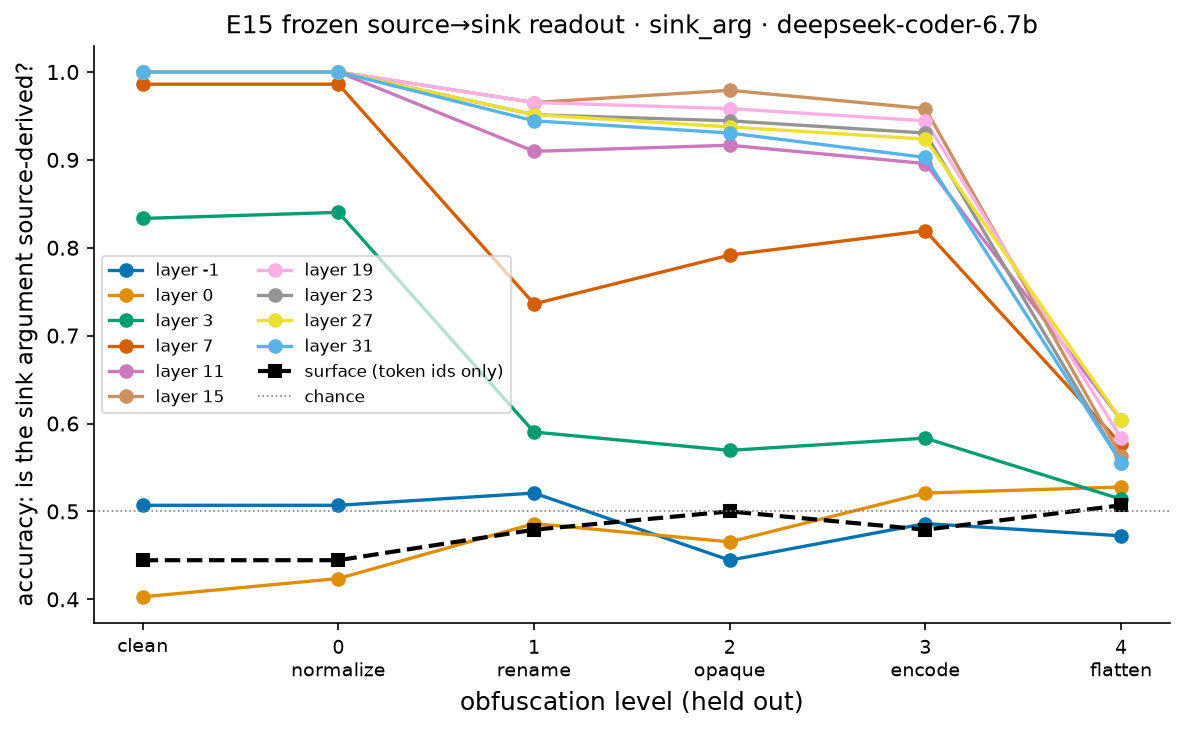
\includegraphics[width=\columnwidth]{../results/figures/sinkflow_levels_deepseek-coder-6.7b.png}
\caption{Source-to-sink readout across DeepSeek-Coder 6.7B layers. The clean condition rises from the embedding floor to ceiling; transformed curves are included for context. Main claims use the frozen selected layer and matched held-out bases.}
\label{fig:depth}
\end{figure}

The controls rule out the specific shortcuts they measure. They do not rule out every regularity of the synthetic generator, nor do they compare the model with a static analyzer designed to compute flow. Our narrow conclusion is that the hidden state makes source-to-sink flow linearly accessible beyond local form, global lexical n-grams, and anchor identity.

\section{Flattening Identifies the Boundary}
\subsection{Atomic attribution}
Table~\ref{tab:atomic} gives the central result. Opaque predicates and MBA encoding independently cost exactly 0.000 in every model. Renaming costs between 0.014 and 0.118, so original identifier names help somewhat but are not required. Flattening is different: by itself it lowers accuracy from 1.000 to 0.688, 0.667, and 0.660. The full four-transformation composition reaches 0.729, 0.653, and 0.674.

\begin{table*}[t]
\centering\small
\caption{Frozen hidden-state accuracy on held-out matched programs. Atomic conditions apply one transformation to normalized code. ``Full'' composes all four.}
\label{tab:atomic}
\begin{tabular}{lcccccc}
\toprule
Model & Clean & Rename & Opaque & MBA & Flatten & Full \\
\midrule
DeepSeek-Coder 1.3B & 1.000 & 0.938 & 1.000 & 1.000 & 0.688 & 0.729\\
DeepSeek-Coder 6.7B & 1.000 & 0.986 & 1.000 & 1.000 & 0.667 & 0.653\\
StarCoder2-3B       & 1.000 & 0.882 & 1.000 & 1.000 & 0.660 & 0.674\\
\bottomrule
\end{tabular}
\end{table*}

The difference between cumulative and atomic flattening is $+0.042$, $-0.014$, and $+0.014$. For comparison, independently drawn rename variants of the same transformation differ by 0.021, 0.035, and 0.028 in absolute accuracy. We therefore do not detect an extra composition penalty beyond ordinary transformation-draw variation. This is stronger and more useful than saying that ``obfuscation hurts'': the readout is robust to dead paths and expression rewrites, mostly robust to changed names, but depends on the structured control-flow scaffold.

\subsection{Why 0.66 is not two-thirds of the relation}
Pooled accuracy can hide a failed paired distinction. Every base has one safe and one unsafe member, so a constant prediction scores 0.5. Under flattening, 51.4\%, 55.6\%, and 45.8\% of matched pairs receive the \emph{same} prediction (Table~\ref{tab:failure}). These pairs no longer expose the intended contrast to the frozen readout.

Formally, our pair-collapse statistic is
\begin{equation}
 C_m(t)=\frac{1}{|\mathcal{B}_{\mathrm{test}}|}
 \sum_{b\in\mathcal{B}_{\mathrm{test}}}
 \mathbb{I}\!\left[
 \hat y_m(T_t(p_b^1))=\hat y_m(T_t(p_b^0))\right].
 \label{eq:collapse}
\end{equation}
Perfect relational discrimination has $C_m(t)=0$. Accuracy and collapse are
not redundant: a readout can achieve above-chance accuracy through a class
bias while assigning the same label to many counterfactual pairs.

The remaining errors also point in different directions. DeepSeek 6.7B labels 66.7\% of programs unsafe, producing unsafe/safe accuracies of 0.833/0.500. StarCoder2 is nearly balanced under atomic flattening, while its full composition shifts toward safe. Similar aggregate scores can therefore arise from different priors. For a paired security property, overall accuracy should be accompanied by class rates and pair collapse.

\begin{table}[t]
\centering\small
\caption{Failure anatomy under atomic flattening. ``Same'' is the fraction of matched safe/unsafe pairs assigned one label.}
\label{tab:failure}
\begin{tabular}{lrrrr}
\toprule
Model & Acc. & Unsafe acc. & Safe acc. & Same\\
\midrule
DS 1.3B & .688 & .625 & .750 & .514\\
DS 6.7B & .667 & .833 & .500 & .556\\
SC2 3B  & .660 & .667 & .653 & .458\\
\bottomrule
\end{tabular}
\end{table}

\subsection{A structural, not uniquely security-specific, limit}
The same rewrite was applied to the project's simpler binding and def--use readouts. At the selected layers, flattening reduces binding accuracy to 0.527--0.615 and def--use accuracy to 0.402--0.545, compared with 0.660--0.688 for source-to-sink flow. Thus the security target is not uniquely fragile. Its failure follows the same boundary as the program relations from which a flow analysis is built.

This comparison also prevents an overclaim. A frozen linear readout may fail because the relation disappears, because it moves to a different basis, or because the source position no longer summarizes a dispatch-loop computation. Our result identifies a loss of \emph{stable linear access} under structural rewriting. It does not prove that all semantic information has been erased.

\section{Decodable Does Not Mean Lexicalized}
The probe answers whether a trained linear boundary can recover the label. A different question is whether the safe-to-unsafe change points toward words the model itself uses for the concept. We map matched hidden-state differences into vocabulary-score space with the standard logit projection and a Jacobian-based local projection (J-lens). For the two DeepSeek models we additionally use a residual-aware projection (R-lens). Candidate security words are chosen on clean training pairs and frozen before held-out evaluation; same-label, orientation-permutation, embedding, and token-identical-site controls are reported in Appendix~\ref{app:lenses}.

Let $g_m:\mathbb{R}^{d_m}\rightarrow\mathbb{R}^{|V_m|}$ denote the model's
final normalization and unembedding map. The logit-lens vocabulary vector is
$z_{m,\ell,s}^{\mathrm{logit}}(p)=g_m(h_{m,\ell,s}(p))$. The J-lens instead
uses a first-order map around the observed state,
\begin{equation}
 z_{m,\ell,s}^{J}(p;\delta h)=
 J_{g_m}(h_{m,\ell,s}(p))\,\delta h,
 \label{eq:jlens}
\end{equation}
and the R-lens propagates the contrast through validated residual-stream rules
before unembedding. For each lens $q$, the matched vocabulary contrast is
\begin{equation}
 d_{b,m,\ell,s}^{q}=z_{m,\ell,s}^{q}(p_b^1)-
 z_{m,\ell,s}^{q}(p_b^0)\in\mathbb{R}^{|V_m|}.
 \label{eq:vocabdiff}
\end{equation}
For a frozen set $V_{\mathrm{sec}}$ of explicit security tokens, we report
the mean contrast
\begin{equation}
 E_{m,\ell,s}^{q}=\frac{1}{|\mathcal{B}_{\mathrm{test}}|}
 \sum_b\sum_{v\in V_{\mathrm{sec}}}d_{b,m,\ell,s,v}^{q}.
 \label{eq:explicit}
\end{equation}
Candidate discovery and orientation use only clean training pairs.

The result is a useful dissociation. First, explicit tokens related to \emph{unsafe}, \emph{tainted}, or \emph{vulnerable} do not consistently receive a positive unsafe-minus-safe contrast. In DeepSeek 1.3B, the explicit-security contrast is significantly inverted. Agreement between projections on the DeepSeek models, and between logit and J-lens across all three models, makes this unlikely to be an artifact of one lens.

Second, a direction built from the full vocabulary-score difference on clean training pairs does generalize. From roughly 25\% depth onward, every one of the 72 held-out unsafe-minus-safe pairs projects positively onto the frozen direction in all three models. The same-label sign rate stays near chance, and the last-token measurement uses an identical token in both pair members. This is evidence for a stable, distributed output-space component of the relation.

For clarity, the training-defined direction and held-out score are
\begin{align}
 v_{m,\ell,s}^{q}
 &=\frac{\sum_{b\in\mathcal{B}_{\mathrm{train}}}d_{b,m,\ell,s}^{q}}
 {\left\|\sum_{b\in\mathcal{B}_{\mathrm{train}}}d_{b,m,\ell,s}^{q}\right\|_2},
 \label{eq:direction}\\
 r_{b,m,\ell,s}^{q}
 &=\left\langle d_{b,m,\ell,s}^{q},v_{m,\ell,s}^{q}\right\rangle .
 \label{eq:projection}
\end{align}
The reported 72/72 result means
$\sum_b\mathbb{I}[r_{b,m,\ell,s}^{q}>0]=72$ on held-out bases, not that a
single vocabulary token separates the classes.

Third, the direction is not a tidy lexical concept. Its largest loadings are spread over arbitrary token fragments, and its singular-value concentration does not clearly exceed the same-label control. We therefore call it a \emph{training-defined distributed direction}, not ``the unsafe feature.'' The label is linearly accessible and leaves a reproducible output-space trace, but the unprompted model does not express it through the obvious security word. Informally, the models represent the distinction more reliably than they name it.

Flattening weakens this distributed projection as well as the hidden-state classifier. Two different measurements therefore locate the same boundary: the output-space organization and the frozen supervised readout both depend on familiar source-level structure.

\section{Discussion}
Taken together, the experiments answer three questions. \textbf{Presence:} source-to-sink flow becomes linearly explicit after contextual computation and is not explained by the measured lexical floors. \textbf{Robustness:} the representation is selective rather than generally fragile; it survives names, dead branches, and MBA form much better than flattened control flow. \textbf{Format:} it is distributed rather than localized on an explicit security token.

This matters for both interpretability and security evaluation. A successful probe on ordinary source can substantially overstate robustness. Conversely, grouping all semantics-preserving rewrites under one ``obfuscated'' condition hides the scientific result: in our benchmark, two transformations are free, one is modest, and one creates the failure. Atomic conditions and matched pairs turn a vague robustness statement into a specific structural diagnosis.

The result also clarifies what semantic understanding should mean here. The models do more than detect dangerous API names: those names and source calls are present in both labels, lexical readers are at chance, and changing identifiers is mostly survivable. Yet the representation is not compiler-normalized, because an equivalent dispatch-loop presentation disrupts access. A useful middle description is that code models build relational summaries adapted to source patterns common in pretraining. Such summaries can support program-analysis tasks, but should not be treated as invariant program semantics.

\paragraph{Limitations.} The benchmark is synthetic Python with three sink families and four flow structures; it is not a malware or real-vulnerability corpus. ``Safe'' denotes a trusted literal at the marked argument and does not model sink-specific sanitization. Whole-program n-grams exclude lexical shortcuts, not an analyzer that computes flow. Frozen linear failure may be a basis change rather than information destruction. Vocabulary alignment is supervised by training labels and observational. Finally, we do not causally intervene on the source-to-sink direction. These limits keep the paper's claim narrow: we audit accessible representations under controlled changes, rather than establish an end-to-end security detector.

\section{Conclusion}
Across three code models, source-to-sensitive-sink flow is constructed contextually and becomes almost perfectly accessible beyond local, global lexical, and embedding controls. Atomic evaluation identifies control-flow flattening as the transformation that breaks this access, while opaque predicates and expression encoding leave it intact and composition adds no detectable penalty. The distinction occupies a reproducible but distributed output-space direction rather than an explicit security word: semantic enough to track flow, but still tied to how source code presents the computation.

\bibliographystyle{plain}
\begin{thebibliography}{10}\scriptsize
\bibitem{boke2025camouflage} E. B\"oke and S. Torka. Digital camouflage: Evaluating code obfuscations against large language models. \emph{arXiv:2509.16671}, 2025.
\bibitem{chen2022cat} Y. Chen et al. CAT-probing: A metric-based approach to interpret how pre-trained models for programming language attend code structure. In \emph{Findings of EMNLP}, 2022.
\bibitem{feng2020codebert} Z. Feng et al. CodeBERT: A pre-trained model for programming and natural languages. In \emph{Findings of EMNLP}, 2020.
\bibitem{guo2021graphcodebert} D. Guo et al. GraphCodeBERT: Pre-training code representations with data flow. In \emph{ICLR}, 2021.
\bibitem{guo2024deepseek} D. Guo et al. DeepSeek-Coder: When the large language model meets programming. \emph{arXiv:2401.14196}, 2024.
\bibitem{hewitt2019control} J. Hewitt and P. Liang. Designing and interpreting probes with control tasks. In \emph{EMNLP-IJCNLP}, 2019.
\bibitem{li2025obfuscation} X. Li et al. A systematic study of code obfuscation against LLM-based vulnerability detection. \emph{arXiv:2512.16538}, 2025.
\bibitem{lozhkov2024starcoder2} A. Lozhkov et al. StarCoder 2 and The Stack v2: The next generation. \emph{arXiv:2402.19173}, 2024.
\bibitem{troshin2022probing} S. Troshin and N. Chirkova. Probing pretrained models of source codes. In \emph{BlackboxNLP}, 2022.
\bibitem{paul2025obscuracoder} R. Paul, K. Yang, G. Glava\v{s}, K. Kersting, and I. Gurevych. ObscuraCoder: Can code language models understand obfuscated code? In \emph{ICLR}, 2025.
\end{thebibliography}

\appendix
\section{Benchmark Details and Validity Gates}\label{app:gates}
The clean set is balanced at every crossing of three families, four structures, and two labels. Generation checks exact pair membership and verifies that train and held-out base identifiers are disjoint. Each generated program must parse, contain exactly one recorded source and one recorded sensitive argument, terminate under restricted execution, and produce a dynamic label equal to the independent AST fixpoint. Transformation manifests record the exact applied set. Every transformed pair must preserve its original label and remain in its original split. Feature extraction additionally checks that every stored character anchor is covered by exactly one token position. A run stops with a named gate failure rather than emitting a headline result if any of these requirements fails.

The final benchmark artifact contains 480 clean programs and 1,296 held-out transformed variants, for 1,776 extracted programs per model. All reported model runs pass gates S0--S3: benchmark integrity, feature coverage, clean grouped-probe validity, and frozen held-out evaluation. The vocabulary analysis passes its candidate-freezing and pair-coverage gates. These checks establish experiment validity; they are not statistical significance tests and do not reject an experiment merely because a scientific effect is small.

\section{Dataset Construction}\label{app:data}
Each base samples names, literals, and harmless surrounding statements independently. Pair members contain the same untrusted source, the same trusted alternative, and the same sink call. The sink argument selects one of the two propagated values. Branch cases assign the selected value through both branch arms; helper cases pass it across one function boundary. This design keeps API presence, program length family, source presence, and sink presence matched while changing flow. Programs are grouped by base for all splits, probe folds, intervals, and pair statistics.

The three families represent command execution, SQL execution, and dynamic code execution. They are useful because they share the same abstract question while differing in surface vocabulary. We do not interpret them as complete models of shell injection, SQL injection, or code injection. In particular, the trusted branch uses a fixed literal rather than a realistic sanitization library, avoiding ambiguous claims about whether a sanitizer is correct for a given sink.

\section{Probe and Statistical Protocol}\label{app:probe}
Hidden states are extracted at the token covering the marked sink argument. A regularized linear classifier is selected by grouped cross-validation on 168 clean training bases. Layer selection is also made only on clean training data: layer 11 for DeepSeek-Coder 1.3B and layer 15 for both DeepSeek-Coder 6.7B and StarCoder2-3B. The resulting classifier is frozen and evaluated on the 72 held-out bases in every condition. No obfuscated example is used to refit a weight, threshold, layer, or token set.

Confidence intervals resample held-out bases, retaining the safe/unsafe pair and all of its variants together. The main analysis emphasizes effect size and replication across models. Accuracy is always supplemented by unsafe accuracy, safe accuracy, predicted-unsafe rate, and the fraction of matched pairs assigned the same label. The latter directly tests whether a readout preserves the within-base contrast.

\begin{table}[h]
\centering\small
\caption{Full atomic flattening results with cluster-bootstrap 95\% confidence intervals.}
\begin{tabular}{lccccc}
\toprule
Model & Accuracy [95\% CI] & Unsafe & Safe & Pred. unsafe & Pair same\\
\midrule
DeepSeek 1.3B & .688 [.618,.750] & .625 & .750 & .438 & .514\\
DeepSeek 6.7B & .667 [.597,.729] & .833 & .500 & .667 & .556\\
StarCoder2-3B & .660 [.583,.736] & .667 & .653 & .507 & .458\\
\bottomrule
\end{tabular}
\end{table}

\section{Controlled Semantic Foundation}\label{app:foundation}
The earlier binding and def--use benchmarks use exact minimal pairs in which token identity, local window, and relevant distance are matched while a relation changes. Their layerwise pattern begins at a declared chance floor and rises after contextual layers. Under the same flattening implementation used here, selected-layer binding accuracy falls to 0.527--0.615 and def--use to 0.402--0.545 across the three models. Source-to-sink flow remains slightly higher at 0.660--0.688, but shares the same qualitative boundary. We include these tasks only as a structural comparison, not as extra contributions of the present paper.

\section{Vocabulary-Space Analysis}\label{app:lenses}
For every matched held-out pair and selected layer, we form an unsafe-minus-safe difference at two sites: the marked sink argument and a token-identical final position. The logit lens applies the model's output normalization and unembedding. The J-lens uses the local Jacobian from the hidden state to vocabulary logits, making the projection conditional on the current computation. The R-lens additionally propagates through validated residual rules. The genuine R-lens is architecture-valid for the two DeepSeek models; StarCoder2 uses the logit and J-lens comparison because its LayerNorm and non-gated MLP do not satisfy the implemented R-lens rules.

Explicit candidate words and any tokenizer-valid variants are discovered on clean training pairs and frozen. Held-out tests compare unsafe-minus-safe probability-mass or score differences against zero and against orientation permutations. Positive-control prompts check that the model can use security vocabulary when the context explicitly asks for a security judgment. Therefore a null unprompted security-word result is not simply evidence that the relevant tokens are impossible for the model to produce.

For the distributed analysis, let $d_i^{(\ell)}$ be the vocabulary-score difference for training pair $i$ at layer $\ell$. We define a unit training direction
\[
v^{(\ell)}=\frac{\sum_i d_i^{(\ell)}}{\left\|\sum_i d_i^{(\ell)}\right\|_2}
\]
and evaluate the sign of $\langle d_j^{(\ell)},v^{(\ell)}\rangle$ on held-out pairs. All 72 held-out pairs have positive projection in each model after approximately one quarter depth. Same-label pairings remain near chance. However, top token loadings are semantically diffuse, and the leading singular-value ratio does not clearly dominate the same-label concentration control. The direction is therefore evidence of reproducible distributed alignment, not evidence for a unique or causal security feature.

All logit- and J-lens analyses have run for DeepSeek-Coder 1.3B, DeepSeek-Coder 6.7B, and StarCoder2-3B. The two DeepSeek models also have the architecture-valid R-lens vocabulary analysis. A separate AST-role relevance redistribution stage exists for 1.3B only and is intentionally excluded from the main argument: its mean permutation result is null and it is not needed for the cross-model conclusion.

\section{Additional Results and Scope}\label{app:extra}
Across structures, assignment chains are the most consistently rename-sensitive condition, but no sink-family ordering replicates strongly enough across models to support a main claim. The paper therefore reports the pooled, pre-registered crossing and uses structure/family rows as diagnostics. Complete machine-readable rows, predictions, manifests, gates, and vocabulary controls are included in the accompanying repository under \texttt{results/sinkflow/<model>/}.

We deliberately leave three questions open. First, a probe trained jointly across structural normal forms could test whether flattening changes the basis rather than removes information. Second, natural vulnerability and malware corpora could test external validity, although they would weaken the exact matching available here. Third, causal interchange or activation patching at the security-flow site would be needed to establish that the decoded relation affects model behavior. These extensions should follow the present diagnosis rather than be mixed into it: the current contribution is the controlled relation, its atomic robustness boundary, and its representational format.

\end{document}
